\section{Teoria della calcolabilità}

\subsection{Sistema di calcolo \texorpdfstring{$\SC$}{C}}
Si vuole modellare matematicamente un calcolatore o sistema di calcolo $\SC$:
\vspace{.4cm}
\begin{figure}[h]
    \centering
    \usetikzlibrary {arrows.meta} 
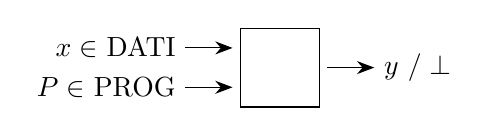
\begin{tikzpicture}

    \draw[-{Stealth[length=2.2mm]}] (2.3,1.75) node[left]{$x\in$\ DATI} -- (2.9,1.75);
    \draw[-{Stealth[length=2.2mm]}] (2.3,1.25) node[left]{$P\in$\ PROG} -- (2.9,1.25);
    \draw (3,2) rectangle (4,1);
    \node at (3.45,1.5) {$\C$};
    \draw[-{Stealth[length=2.2mm]}] (4.1,1.5) -- (4.7,1.5)
        node [right] {$y\ /\perp$};

\end{tikzpicture}
\end{figure}

La figura mostra il sistema di calcolo $\SC$ che, preso un programma $P$
su input $x$, restituisce in output il risultato $y$ o il valore $\perp$
se il programma va in loop.

DATI è l'insieme di tutti i possibili dati di input e PROG l'insieme di
tutti i possibili programmi.

Il sistema di calcolo $\SC$ non fa altro che eseguire il programma $P$ su input
$x$ ricavandone il risultato $y$:
\begin{equation}\label{eq:sistema_calcolo}
\SC:\text{PROG}\times\text{DATI}\rightarrow\text{DATI}_\perp
\end{equation}

Quello che fa il programma $P$ è trasformare il dato di input $x$ in un dato
di output $y$; si può quindi dire che un programma non è altro che
una funzione che agisce da DATI in DATI:
$$ P:\text{DATI} \rightarrow \text{DATI}_\perp $$
$$ \Downarrow $$
\begin{equation}\label{eq:prog_dati} \text{PROG} =
\text{DATI}^{\text{DATI}}_\perp \end{equation}

La funzione associata al programma $P$ è detta \textbf{semantica di $P$}.

Da (\ref{eq:sistema_calcolo}) e (\ref{eq:prog_dati}) si ottiene che:
$$ \SC:\text{DATI}^{\text{DATI}}_\perp\times\text{DATI}
\rightarrow\text{DATI}_\perp $$

$\SC$ è una funzione di valutazione; $\SC(P,x)$ è infatti la semantica di $P$.

\subsection{Potenza computazionale di \texorpdfstring{$\SC$}{C}
\label{sec:pot_comp}}
Si definisce potenza computazionale di $\SC$:
$$ F(\SC) = \{\SC(P,\_):P\in\text{PROG}\} \subseteq \text{DATI}^{\text{DATI}}_\perp $$
\textbf{$F(\SC)$ contiene tutto ciò che un qualsiasi sistema di calcolo $\SC$
può calcolare}. Quindi, per stabilire cosa l'informatica può risolvere, basta stabilire
il carattere dell'inclusione:
\begin{itemize}
    \item $F(\SC)\subset\text{DATI}^{\text{DATI}}_\perp \Rightarrow $
        esistono problemi che l'informatica non può risolvere;
    \item $F(\SC)=\text{DATI}^{\text{DATI}}_\perp \Rightarrow $
        l'informatica può risolvere tutto.
\end{itemize}

\subsection{Cardinalità di insiemi infiniti}
Per riuscire a capire se l'inclusione
$F(\SC)\subseteq\text{DATI}^{\text{DATI}}_\perp$ sia propria o meno, si confronterà
la cardinalità dei due insiemi. Infatti dalla cardinalità si può ricavare che:
\begin{itemize}
    \item Se $|F(\SC)|<\left|\text{DATI}^{\text{DATI}}_\perp\right|
    \quad \Rightarrow \quad F(\SC)\subset\text{DATI}^{\text{DATI}}_\perp$;
    \item Se $|F(\SC)|=\left|\text{DATI}^{\text{DATI}}_\perp\right|
    \quad \Rightarrow \quad F(\SC)=\text{DATI}^{\text{DATI}}_\perp$.
\end{itemize}

Il concetto di cardinalità è semplice quando si tratta di insiemi finiti: basta
contare il numero di elementi che compongono l'insieme. Tuttavia, in presenza
di insiemi infiniti le cose si complicano.

Per esempio, si confrontino $\N$ e $\RN$: entrambi hanno cardinalità infinita
($|\N|=|\RN|=\infty$) eppure $\N\subset\RN$! Per comprendere quindi meglio
la cardinalità di insiemi infiniti si dovrà andare più nel dettaglio.

\subsubsection{Relazione binaria}
Si definisce relazione binaria $R$ sull'insieme $A$, un elenco di coppie ordinate
di elementi di $A$: $R\subseteq A^2$. Due elementi $a,b\in A$ sono in relazione 
$R$ se $(a,b)\in R$. Si usa la notazione:
\begin{itemize}
    \item $a \ R \ b$: $a$ è in relazione $R$ con $b$;
    \item $a\ \cancel{R} \ b$: $a$ non è in relazione $R$ con $b$;
\end{itemize}

\subsubsection{Relazione di equivalenza}
$R\subseteq A^2$ è una relazione di equivalenza se gode di:
\begin{enumerate}
    \item Riflessività: $\forall a \in A \quad a \ R \ a$
    \item Simmetria: $\forall a,b \in A \quad a \ R \ b \ \Leftrightarrow \ b \ R \ a$
    \item Transitività: $\forall a,b,c \in A \quad a \ R \ b
    \ \wedge \ b \ R \ c \Rightarrow a \ R \ c $
\end{enumerate}

\subsubsection{Classe di equivalenza}
Si definisce classe di equivalenza $[a]_R$ l'insieme degli elementi in relazione $R$
con $a$:
$$ [a]_R =\{b\in A: a \ R \ b\} $$

Tutte le classi di equivalenza di $R$ formano una partizione di $A$. L'insieme $A$
partizionato attraverso le classi di equivalenza di $R$ è detto \textbf{quoziente}
di $A$ rispetto a $R$ ed è denotato da $\sfrac{A}{R}$.

\subsubsection*{Esempio}
Si consideri la relazione $\equiv_4\subseteq\N^2$ di equivalenza modulo 4. Due numeri
sono in relazione di equivalenza modulo 4 se il resto della divisione per 4 è uguale
per entrambi.
$$ 5\equiv_4 9\ , \ 10\equiv_4 2 \ , \ \dots $$

Le classi di equivalenza sono:
\begin{align}
    [0]_4&=\{4k\}\tag{Multipli di 4}\\
    [1]_4&=\{4k+1\}\tag{Resto 1}\\
    [2]_4&=\{4k+2\}\tag{Resto 2}\\
    [3]_4&=\{4k+3\}\tag{Resto 3}
\end{align}
L'insieme $\{[0]_4,[1]_4,[2]_4,[3]_4\}=\sfrac{\N}{\equiv_4}$ è una partizione di $\N$.

\subsubsection{Insiemi isomorfi}
Due insiemi $A$ e $B$ sono \textbf{isomorfi} (o equinumerosi) se esiste una funzione
biettiva tra essi. Formalmente si indica con:
$$ A\sim B $$
La relazione di isomorfismo $\sim$ è una relazione di equivalenza in quanto:
\begin{enumerate}
    \item Riflessiva: si usi la funzione identità;
    \item Simmetrica: se esiste una funzione biettiva allora anche la sua inversa
        è biettiva;
    \item Transitiva: la composizione di due funzioni biettive è una funzione biettiva.
\end{enumerate}

Sia $\mathscr{U}$ l'insieme universo, ovvero l'insieme che contiene tutti gli insiemi.
Il quoziente di $\mathscr{U}$ rispetto a $\sim$ ($\sfrac{\mathscr{U}}{\sim}$) definisce il 
concetto di cardinalità:

\begin{figure}[H]
    \centering
    \begin{tikzpicture}[scale=1.5]

    \node at (-2,1) {$\sfrac{\mathscr{U}}{\sim}$};

    \draw[thick] (0,0) node{...} ellipse (2 and 1);
    \draw (-1.25,-.78) -- (-1.25,.78);
    \draw (-.5,-.97) -- (-.5,.97);
    \draw (.5,-.97) -- (.5,.97);
    \draw (1.25,-.78) -- (1.25,.78);

    \draw[fill,blue] (-.875,0) circle (.02);
    \draw[->,blue] (-.875,0) -- (-1.75,-1);
    \node[blue,below] at (-1.75,-1) {Classe di equivalenza};

\end{tikzpicture}
\end{figure}

Ogni partizione di $\sfrac{\mathscr{U}}{\sim}$ contiene gli insiemi tra loro isomorfi, ovvero
che hanno la stessa cardinalità.

\subsubsection*{Insiemi finiti}
Si definisca la famiglia di insiemi: 
$$J_n=\begin{cases}
\cancel{O} & n=0\\
\{1,\dots ,n\} & n>0
\end{cases}$$
$$ J_0=\{\}\ , \ J_1=\{1\} \ , \ J_{2}=\{1,2\} \ , \ J_{3}=\{1,2,3\}\ , \ \dots $$

Un'insieme $A$ ha cardinalità finita se $\exists n\in\N : A\sim J_n$ e si può dire che
$|A|=n$.

\subsubsection*{Insiemi infiniti}
Un insieme che non è finito ha cardinalità infinita.

\subsubsection{Insiemi numerabili}
Un insieme $A$ è numerabile se $\N\sim A$ (ovvero $A\in [\N]_\sim$). Vuole quindi dire
che esiste una biezione $f:\N\rightarrow A$ che permette di listare $A$ come:
$$ A = \{f(0),f(1),f(2),\dots\} $$
senza tralasciare nessun elemento.
\subsubsection*{Esempi}
\begin{tabular}{r l}
    PARI :& $f(n)=2n$ \\
    DISPARI :& $f(n)=2n+1$ \\
    $\mathbb{Z}$ :& mappo i pari nei non-negativi e i dispari nei negativi \\
    $\{0\}\cup 1\{0,1\}^*$ :& converto da binario a decimale \\
\end{tabular}

\subsubsection{Insiemi non numerabili}
Gli insiemi non numerabili sono insiemi a cardinalità infinita ma non listabili come
$\N$ (sono \quotes{più fitti}). Il re di questi insiemi è $\RN$.

\begin{theorem}
    $\RN$ è un insieme non numerabile: $$ \N \nsim \RN $$
\end{theorem}
\begin{proof} Per dimostrarlo dimostro che:
    \begin{enumerate}
        \item $\RN \sim (0,1)$: la biezione è rappresentata graficamente in figura:
            \vspace{-.2cm}
            \begin{figure}[H]
                \centering
                \begin{tikzpicture}[scale=2]

    \draw (-1.7,0) -- (1.7,0);
    \draw[densely dashed] (-1.7,0) -- (-2,0);
    \draw[densely dashed] (1.7,0) -- (2,0);
    \draw (0,.05) -- (0,-.05) node[below] {0};
    
    \draw[cyan] (1,1.5) arc[start angle=0, end angle=-180,radius=1];

    \draw (-1,1.5) -- (1,1.5);
    \draw (-1,1.55) -- (-1,1.45) node[left] {0};
    \draw (1,1.55) -- (1,1.45) node[right] {1};

    \draw[densely dashed, cyan] (-.515,.64) --  (0,1.5);
    \draw[red] (-.9,0) -- (-.515,.64) -- (-.515,1.5);
    \draw (-.515,1.45) -- (-.515,1.55) node[above] {$f(a)$};
    \draw (-.9,.05) -- (-.9,-.05) node[below] {$a$};

    \draw[densely dashed, cyan] (.68,.77) -- (0,1.5);
    \draw[red] (1.4,0) -- (.68,.77) -- (.68,1.5);
    \draw (.68,1.45) -- (.68,1.55) node[above] {$f(b)$};
    \draw (1.4,.05) -- (1.4,-.05) node[below] {$b$};

    \draw [fill] (0,1.5) circle (.02);

\end{tikzpicture}
            \end{figure}\vspace{-.6cm}
            (In realtà $\RN$ è isomorfo a un suo qualsiasi intervallo).
        \item $\N \nsim (0,1)$: dimostrazione per assurdo: assumo che $\N \sim (0,1)$;
            Questo vorrebbe dire che tutti i numeri compresi tra 0 e 1 sono numerabili.
            Elenco tutti i numeri associandoli a un numero naturale:

            \begin{minipage}{.45\textwidth}
                $$0\ \mapsto \ 0.{\color{red}a_{00}}\ a_{01}\ a_{02}\ a_{03}\ a_{04}\ \dots$$
                $$1\ \mapsto \ 0.a_{10}\ {\color{red}a_{11}}\ a_{12}\ a_{13}\ a_{14}\ \dots$$
                $$2\ \mapsto \ 0.a_{20}\ a_{21}\ {\color{red}a_{22}}\ a_{23}\ a_{24}\ \dots$$
                $$3\ \mapsto \ 0.a_{30}\ a_{31}\ a_{32}\ {\color{red}a_{33}}\ a_{34}\ \dots$$
                $$4\ \mapsto \ 0.a_{40}\ a_{41}\ a_{42}\ a_{43}\ {\color{red}a_{44}}\ \dots$$
                $$\vdots\qquad\vdots\qquad\vdots\qquad\vdots\qquad\vdots\qquad\ddots$$
                \vspace{.4cm}
            \end{minipage}
            \begin{minipage}{.48\textwidth}
                $a_{ij}$ è la $i$-esima cifra dopo lo zero del $j$-esimo numero
                nella lista.

                Se $(0,1)$ fosse numerabile tutti i suoi numeri dovrebbero far parte
                della lista.

                Si consideri il numero:
                $$ 0.c_0c_1c_2c_3\dots $$

                con: $$ c_i = \begin{cases}
                2 & a_{ii}\neq2\\
                3 & a_{ii}=2
                \end{cases} $$

            \end{minipage}
            Chiaramente $0.c_0c_1c_2c_3\dots\in(0,1)$ ma non appare nella lista:
            \begin{itemize}
                \item Differisce dal primo numero perchè $c_0\neq a_{00}$;
                \item Differisce dal secondo numero perchè $c_1\neq a_{11}$;
                \item $\dots$
                \item Differisce da qualunque numero nella lista sulla cifra 
                    {\color{red} diagonale}.
            \end{itemize}
            Ho trovato l'assurdo quindi $\N \nsim (0,1)$ (dimostrazione per 
            diagonalizzazione).
    \end{enumerate}
    Sfruttando la transitività di $\sim$ posso si può affermare quindi che:
    $$ \RN \underset{(1)}{\sim} (0,1) \underset{(2)}{\nsim} \N \quad \Rightarrow \quad \RN \nsim \N $$
\end{proof}

Tutti gli insiemi isomorfi a $\RN$ sono detti continui. Altri insiemi non numerabili sono:
\begin{itemize}
    \item $2^\N\nsim\N$: insieme delle parti di $\N$ ovvero $2^\N = \{\text{sottoinsiemi di } \N\}$
    \item $\N^\N_\perp\nsim\N$: insieme delle funzioni da $\N$ a $\N$ ovvero
        $\N^\N_\perp = \{f:\N\rightarrow\N_\perp\}$
\end{itemize}

\subsection{Esistono funzioni non calcolabili?}
Ora che il concetto di cardinalità è più chiaro, si riprenda il concetto di 
potenza computazionale di un sistema di calcolo $\SC$ (paragrafo \ref{sec:pot_comp}):
$$
F(\SC) = \{\SC(P,\_):P\in\text{PROG}\} \subseteq \text{DATI}^{\text{DATI}}_\perp
$$

Per definizione $F(\SC)$ ha la stessa numerosità di PROG:
$$ F(\SC) \sim \text{PROG} $$

Ragionevolmente, \textbf{ma non formalmente}, si può notare che:
\begin{itemize}
    \item PROG$\sim\N$: si prenda la stringa binaria con la quale il programma è
        salvato sul disco e si converta da binario a decimale;
    \item DATI$\sim\N$: si applichi lo stesso ragionamento del punto precedente.
\end{itemize}
Ne segue che:
$$ F(\SC) \sim \text{PROG} \sim \N \nsim\N^\N_\perp\sim \text{DATI}^\text{DATI}_\perp$$
$$ \Downarrow $$
$$ F(\SC) \nsim \text{DATI}^\text{DATI}_\perp $$
$$ \Downarrow $$
$$ F(\SC) \subset \text{DATI}^\text{DATI}_\perp $$

Quello che questa osservazione dice è che ho pochi programmi ($\N$) e troppe
funzioni ($\N^\N_\perp$).
\textbf{Alla domanda \quotes{Esistono funzioni non calcolabili?} si può quindi 
rispondere con un sì!}

\subsection{\texorpdfstring{DATI$\bm{\sim\N}$}{DATI~N}}
Obiettivo di questa sezione è dimostrare formalmente che:
$$ \text{DATI} \sim \N $$
Vogliamo quindi trovare una biezione che è in grado di associare biunivocamente
dei dati a un numero e quindi anche di ottenere i dati di partenza dal
numero. Per farlo si userà il seguente teorema.

\begin{theorem}
    $\N\times\N\sim\N^+$
\end{theorem}
\begin{proof}
    Si definisca la funzione coppia di Cantor $\cantor{\ ,\ }$:
    $$ \cantor{\ ,\ }:\N\times\N\rightarrow\N^+ $$
    $\cantor{\ ,\ }$ associa biunivocamente una coppia di numeri $x$ e 
    $y$ a un numero $n$:
    $$ \cantor{x,y} = n $$
    La mappa che $\cantor{\ ,\ }$ usa per assegnare i valori di ogni coppia viene 
    descritta nelle seguenti tabelle:

    \begin{minipage}{.48\textwidth}
        \centering
        \begin{tabular}{c|c c c c c c}
            $x\backslash y$&0 &1 &2 &3 &4\\ \hline
               0 &1 &3 &6 &10&15\\
               1 &2 &5 &9 &14&...\\
               2 &4 &8 &13&...&  \\
               3 &7 &12&...&  &  \\
               4 &11&...&  &  &  \\
               5 &$\nearrow$&&&&\\
        \end{tabular}
    \end{minipage}
    \begin{minipage}{.48\textwidth}
        \centering
        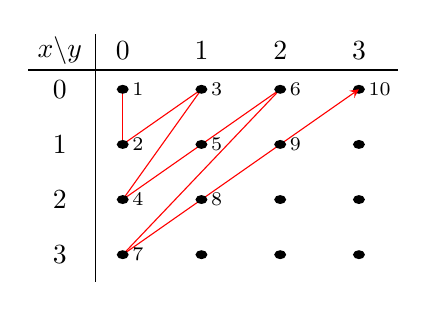
\begin{tikzpicture}[yscale=.7]
    \usetikzlibrary{arrows.meta}

    \tikzset{
        myarrow/.style=-stealth
    }

    \foreach \x in {0,1,2,3} {
        \node at (.2,-\x-1) {\x};
    }
    \foreach \y in {0,1,2,3} {
        \node at (\y+1,-.3) {\y};
    }
    \draw[red] (1,-1) -- (1,-2);
    \draw[red] (1,-2) -- (2,-1);
    \draw[red] (2,-1) -- (1,-3);
    \draw[red] (1,-3) -- (3,-1);
    \draw[red] (3,-1) -- (1,-4);
    \draw[red] (1,-4) -- (3+.2,-2+.2);

    \node at (.2,-.3) {$x\backslash y$};
    \foreach \x in {0,1,2,3} {
        \foreach \y in {0,1,2,3} {
            \ifthenelse{\x<\y \OR \x=\y}{
                \draw[thick,fill] (4-\y,-\x-1) circle (.06);
            }{}
        }
    }
    \draw[myarrow,red] (3+.2,-2+.2) -- (4,-1);
    \node[right] at (1,-1) {\scriptsize 1};
    \node[right] at (1,-2) {\scriptsize 2};
    \node[right] at (2,-1) {\scriptsize 3};
    \node[right] at (1,-3) {\scriptsize 4};
    \node[right] at (2,-2) {\scriptsize 5};
    \node[right] at (3,-1) {\scriptsize 6};
    \node[right] at (1,-4) {\scriptsize 7};
    \node[right] at (2,-3) {\scriptsize 8};
    \node[right] at (3,-2) {\scriptsize 9};
    \node[right] at (4,-1) {\scriptsize 10};

    \draw (-.2,-.65) -- (4.5,-.65);
    \draw (.65,0) -- (.65,-4.5);

\end{tikzpicture}
    \end{minipage}

    Si vuole calcolare ora la forma analitica di $\cantor{\ ,\ }$; si prenda una generica
    coppia di numeri $\cantor{x,y}$:

    \begin{minipage}{.4\textwidth}
        \centering
        \begin{tikzpicture}[yscale=.8]
    \usetikzlibrary{arrows.meta}

    \newcommand{\smallerplus}{\raisebox{.3\height}{\scalebox{.6}{+}}}

    \draw[red,densely dashed] (1,-4) -- (3,-2);
    \draw[densely dashed] (.65,-2) -- (3,-2);
    \draw[densely dashed] (3,-1+.2) -- (3,-2);

    \node at (.1,-.3) {$x\backslash y$};

    \node at (2+1,-.3) {$y$};
    \node at (.9,-.3) {0};
    \node at (1+1,-.3) {$\dots$};
    \node at (.1,-1) {$\vdots$};
    \node at (.1,-1-1) {$x$};
    \node at (.1,-2-1) {$\vdots$};
    \node at (.05,-3-1-.05) {$x{\color{red}\smallerplus y}$};
    \def \offset {.28}
    \draw[white,fill] (3-\offset-.15,-2-\offset) rectangle (3+\offset+.05,-2+\offset-.05);
    \node at (3,-2) {$\cantor{x,y}$};
    \draw[white,fill] (1-\offset-.15,-4-\offset) rectangle (1+\offset+.05,-4+\offset-.05);
    \node[blue] at (1.1,-4) {$\cantor{x\smallerplus y,0}$};

    \draw (-.2,-.65) -- (4.5,-.65);
    \draw (.45,0) -- (.45,-4.5);

\end{tikzpicture}
    \end{minipage}
    \begin{minipage}{.58\textwidth}
        Per come è definita $\cantor{x,y}$ (vedi tabella precedente) si ha che:
        \begin{equation}\label{eq:cantor_analytic}
            \cantor{x,y} = {\color{blue}\cantor{x+y,0}}{\color{red}+y}
        \end{equation}

        Ora l'incognita da calcolare resta $\color{blue}\cantor{z,0}$ che,
        si può ottenere come:
        \begin{equation}\label{eq:cantor_analytic_2}
            \cantor{z,0} = \sum_{i=0}^z i+1 = \frac{z(z+1)}{2}+1
        \end{equation}
    \end{minipage}
    
    Da (\ref{eq:cantor_analytic}) e (\ref{eq:cantor_analytic_2}) segue che:
    $$ \cantor{x,y} = \cantor{x+y,0}+y = \frac{(x+y)(x+y+1)}{2}+y+1 $$
    
    $\cantor{\ ,\ }$ si dimostra quindi mappare univocamente le coppie di numeri
    in numeri ($\N^2\rightarrow\N^+$). Si cercherà ora di mostrare il passaggio inverso, 
    ovvero come riottenere la coppia di numeri dal numero risultante
    ($\N^+\rightarrow\N^2$).

    Si definiscano le seguenti funzioni:
    $$ \cantor{x,y} = n \quad , \quad \sx(n) = x \quad , \quad \dx(n) = y $$

    Da (\ref{eq:cantor_analytic}) si ha che:
    $$ \begin{aligned}
        y &= \cantor{x,y}-\cantor{x+y,0} \\
          &= n-\cantor{x+y,0} \\
          &= n-\cantor{\gamma,0} \\
    \end{aligned} $$
    Il valore di $\gamma$ è il più grande valore che, messo sulla prima colonna
    ($\cantor{\gamma,0}$), non supera $n$:
    $$ \gamma = \max\{z\in\N:\cantor{z,0}\leq n\} $$
    $$ \cantor{z,0}\leq n $$
    $$ \frac{z(z+1)}{2}+1 \leq n $$
    $$ z^2+z+2-2n\leq 0 $$
    $$ \frac{-1-\sqrt{8n-7}}{2}\leq z \leq \frac{-1+\sqrt{8n-7}}{2} $$
    $$ \Downarrow $$
    $$ \gamma=\left\lfloor\frac{-1+\sqrt{8n-7}}{2}\right\rfloor $$
    
    In conclusione:
    $$ \dx(x) = n-\cantor{\gamma,0} $$
    \begin{equation} \sx(x) = \gamma-des(x) \tag{non è il seno} \end{equation}

    La funzione coppia di Cantor $\cantor{\ ,\ }$ si è quindi mostrata
    essere una biezione tra $\N^+$ e $\N^2$, mostrando che i due insiemi
    hanno la stessa cardinalità.
\end{proof}

È facile poi, partendo da $\cantor{\ ,\ }$, creare una biezione tra $\N$ e $\N^2$
(dimostrando che $\N\times\N\sim\N$):
$$ [\ ,\ ]:\N\times\N\rightarrow\N $$
$$ [x,y] = \cantor{x,y}-1 $$

Il precedente risultato mette alla luce anche che:
$$ \mathbb{Q}\sim\N $$
in quanto ogni suo elemento non è altro che una coppia di numeri messi
a frazione.

Ora che si ha appurato l'esistenza di una biezione tra coppie di numeri e numeri si può
facilmente estendere questa relazione a liste d'interi, dove con lista si intende una
sequenza di numeri di lunghezza non nota:
$$ x_1,x_2,\dots,x_m \rightarrow \cantor{x_1,x_2,\dots,x_m} $$
Per farlo basterà applicare $\cantor{\ ,\ }$ come segue:
$$ \cantor{x_1,x_2,\dots,x_m} = 
\cantor{x_1,\cantor{x_2,\cantor{\dots,\cantor{x_m,0}\dots}}} $$
Dove lo 0 a destra della coppia di Cantor più interna rappresenta il fine lista.

La decodifica invece avverrà nel seguente modo:
\begin{figure}[H]
    \centering
    \begin{tikzpicture}[
    level distance=13mm,
    sibling distance=30mm,
]
    \node {\Large$n_0$} 
        child {node[blue] {\Large$x_1$} 
            edge from parent node[xshift=-3,yshift=4,rotate=40.8] {\scriptsize$\sx(n_0)$}
        }
        child {node {\Large$n_1$}
            child {node[blue] {\Large$x_2$}
                edge from parent node[xshift=-3,yshift=4,rotate=40.8] {\scriptsize$\sx(n_1)$}  
            }
            child {node {\Large$n_2$}
                child {node[blue] {\Large$\phantom{n_1}\dots\phantom{n_1}$}
                    edge from parent node[xshift=-3,yshift=4,rotate=40.8] {\scriptsize$\sx(n_2)$}  
                }
                child {node {\Large$\phantom{n_1}\dots\phantom{n_1}$}
                    child {node[blue] {\Large$x_m$}
                        edge from parent node[xshift=-3,yshift=4,rotate=40.8] {\scriptsize$\sx(n_{m-1})$}  
                    }
                    child {node {\Large$0$} edge from parent 
                        node[xshift=3,yshift=4,rotate=-40.8] {\scriptsize$\dx(n_{m-1})$}}
                    edge from parent node[xshift=3,yshift=4,rotate=-40.8] {\scriptsize$\dx(n_2)$}
                }
                edge from parent node[xshift=3,yshift=4,rotate=-40.8] {\scriptsize$\dx(n_1)$}
            }
            edge from parent node[xshift=3,yshift=4,rotate=-40.8] {\scriptsize$\dx(n_0)$}
        };
\end{tikzpicture}
\end{figure}

Qualsiasi tipo di dato può essere convertito a una lista di numeri:
\begin{itemize}
    \item Testi: non sono altro che liste di caratteri i quali possono essere convertiti
        in numeri tramite tabella ASCII;
    \item Suoni: si usa un campionamento a una data frequenza ottenendo una lista di
        valori;
    \item Matrici: una matrice è una lista di liste;
    \item Immagini: ogni pixel contiene la codifica numerica di un colore; in questo modo
    un'immagine non è altro che una matrice di numeri grande quanto la sua risoluzione;
    \item Grafi: uso liste o matrici di adiacenza.
\end{itemize}

\textbf{Si può quindi affermare che $\bm{\text{DATI}\sim\N}$}.

\subsection{\texorpdfstring{PROG$\bm{\sim\N}$}{PROG~N}}
Obiettivo di questa sezione è dimostrare formalmente che:
$$ \text{PROG} \sim \N $$
Per poterlo fare si dovrà definire formalmente un sistema di calcolo specifico: il sistema 
di calcolo RAM, composto dalla macchina RAM e il linguaggio RAM. Quest'ultimo si può 
riassumere come un assembly molto semplificato.

L'idea è di usare il sistema RAM come rappresentativo di tutti i possibili sistemi di calcolo;
ne segue che $F(\RAM)$, ovvero la potenza computazionale di un sistema RAM, permetterà
di capire cosa i sistemi di calcolo sono in grado di calcolare.

Può però sorgere spontaneo un dubbio: il sistema RAM non è troppo semplice per rappresentare
tutti i sistemi di calcolo? Se il sistema RAM non fosse in grado di risolvere
certi problemi, magari altri sistemi più complessi lo sarebbero.

Per verificare questo caso si vedrà successivamente un altro sistema di calcolo più
sofisticato: quello WHILE. Il confronto tra le due potenze computazionali porterebbe a:
\begin{itemize}
    \item $F(\WHILE)\neq F(RAM) \Rightarrow$ la computabilità dipende dallo strumento usato;
    \item $F(\WHILE)=F(RAM) \Rightarrow$ la computabilità è intrinseca nei problemi 
        (tesi di Church-Turing).
\end{itemize}

\subsubsection{Sistema di calcolo RAM}
\subsubsection*{Macchina RAM}
\begin{figure}[H]
    \centering
    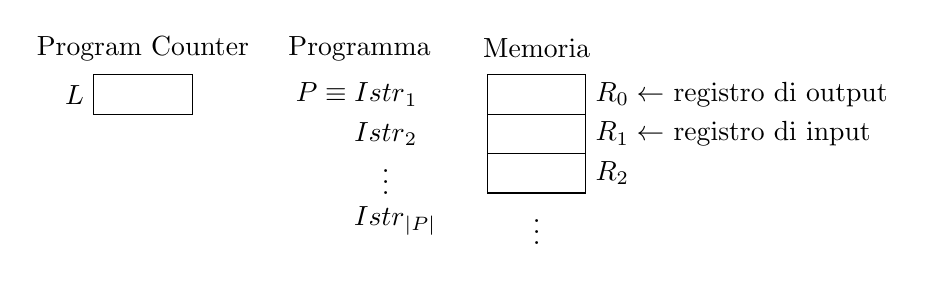
\begin{tikzpicture}
    \node[above] at (.875,.6) {Memoria};

    \draw (.25,0) rectangle (1.5,.5);
    \node[right] at (1.5,.25) {$R_0 \leftarrow$ registro di output};
    \draw (.25,-.5) rectangle (1.5,0);
    \node[right] at (1.5,-.25) {$R_1 \leftarrow$ registro di input};
    \draw (.25,-1) rectangle (1.5,-.5);
    \node[right] at (1.5,-.75) {$R_2$};
    
    \node[below] at (.875,-1) {$\vdots$};

    \def\y{2.25}
    \node[above] at (.875-\y,.55) {Programma};
    \node[] at (.84-\y,.25) {$P\equiv\text{Istr}_1$};
    \node[] at (1.21-\y,-.25) {$\text{Istr}_2$};
    \node[] at (1.21-\y,-.75) {$\vdots$};
    \node[] at (1.33-\y,-1.35) {$\text{Istr}_{|P|}$};

    \def\x{5}
    \node[above] at (.875-\x,.55) {Program Counter};

    \draw (.25-\x,0) rectangle (1.5-\x,.5);
    \node[left] at (1.5-1.25-\x,.25) {$L$};
\end{tikzpicture}
\end{figure}
\begin{itemize}
    \item $L$ contiene l'indirizzo della prossima istruzione da eseguire ($1\leq L\leq |P|$)
    \item $P$ è il programma ovvero una lista di istruzioni $\text{Istr}_i$
    \item $R_i$ è un generico registro di memoria che può contenere un numero naturale:
    \begin{itemize}
        \item $R_0$ è il registro specifico dove verrà deposto l'output del programma
        \item $R_1$ è il registro specifico dove verrà letto l'input del programma
        \item Il numero dei registri è illimitato
    \end{itemize}
\end{itemize}
\subsubsection*{Linguaggio RAM}
La sintassi del linguaggio RAM è molto intuitiva; ci sono tre tipi di istruzioni:

\begin{minipage}{.4\textwidth}
    \begin{enumerate}
        \itemsep.5em 
        \item $R_k \leftarrow R_k +1$ 
        \item $R_k \leftarrow R_k \dotminus 1$
        \item $\goto{R_k}{m}$
    \end{enumerate}
\end{minipage}
\begin{minipage}{.49\textwidth}
    $$x\dotminus y =\begin{cases}x-y&x\geq y\\ 0 &\text{altrimenti}\end{cases}$$
\end{minipage}

Si noti che il numero di istruzione $m$ usato nel terzo comando deve essere compreso tra
1 e $|P|$ inclusi.

\subsubsection*{Esecuzione}
Per eseguire un programma $P$ su input $\color{red}n$ la macchina verrà inizializzata come segue:
\begin{figure}[H]
    \centering
    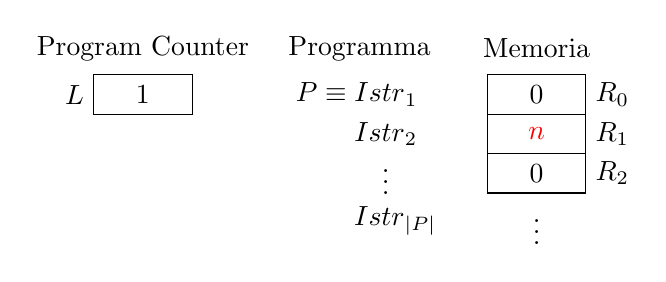
\begin{tikzpicture}
    \node[above] at (.875,.6) {Memoria};

    \draw (.25,0) rectangle (1.5,.5) node[midway] {$0$};
    \node[right] at (1.5,.25) {$R_0$};
    \draw (.25,-.5) rectangle (1.5,0) node[midway] {$\color{red}n$};
    \node[right] at (1.5,-.25) {$R_1$};
    \draw (.25,-1) rectangle (1.5,-.5) node[midway] {$0$};
    \node[right] at (1.5,-.75) {$R_2$};
    
    \node[below] at (.875,-1) {$\vdots$};

    \def\y{2.25}
    \node[above] at (.875-\y,.55) {Programma};
    \node[] at (.84-\y,.25) {$P\equiv\text{Istr}_1$};
    \node[] at (1.21-\y,-.25) {$\text{Istr}_2$};
    \node[] at (1.21-\y,-.75) {$\vdots$};
    \node[] at (1.33-\y,-1.35) {$\text{Istr}_{|P|}$};

    \def\x{5}
    \node[above] at (.875-\x,.55) {Program Counter};

    \draw (.25-\x,0) rectangle (1.5-\x,.5) node[midway] {$1$};
    \node[left] at (1.5-1.25-\x,.25) {$L$};
\end{tikzpicture}
\end{figure}

Successivamente si eseguirà un'istruzione dopo l'altra, a partire dalla prima, facendo quindi
incrementare di uno il program counter ($L\leftarrow L+1$) dopo l'esecuzione di ogni istruzione.
Se l'istruzione è un'istruzione di salto ($\goto{R_k}{m}$) e la sua condizione $R_k=0$
è verificata, il program counter verrà cambiato in $L\leftarrow m$.

Per convenzione $L=0 \Rightarrow \text{ Fine del programma}$ (con possibiliità di loop infinito).

L'output del programma sarà il contenuto di $R_0$ o $\perp$ in presenza di loop.

\subsubsection*{Semantica operazionale}
La semantica operazionale descrive formalmente il significato di ogni istruzione; per farlo
specifica l'effetto che l'istruzione ha sui registri della macchina.

L'esecuzione di un programma è una sequenza di stati della macchina, dove uno stato descrive
precisamente l'attuale situazione della macchina. Ogni istruzione fa passare la macchina da
uno stato ad un altro:
$$ \text{STATO}_1 \rightarrow \boxed{\text{Istr}_i} \rightarrow \text{STATO}_2 $$
$$ (\text{STATO}_1,\text{STATO}_2) = \text{semantica operazionale di Istr}_i $$

Ampliando il concetto di semantica dalla singola istruzione all'intero programma si ha che 
quest'ultimo induce una sequenza di stati:
\begin{figure}[H]
    \centering
    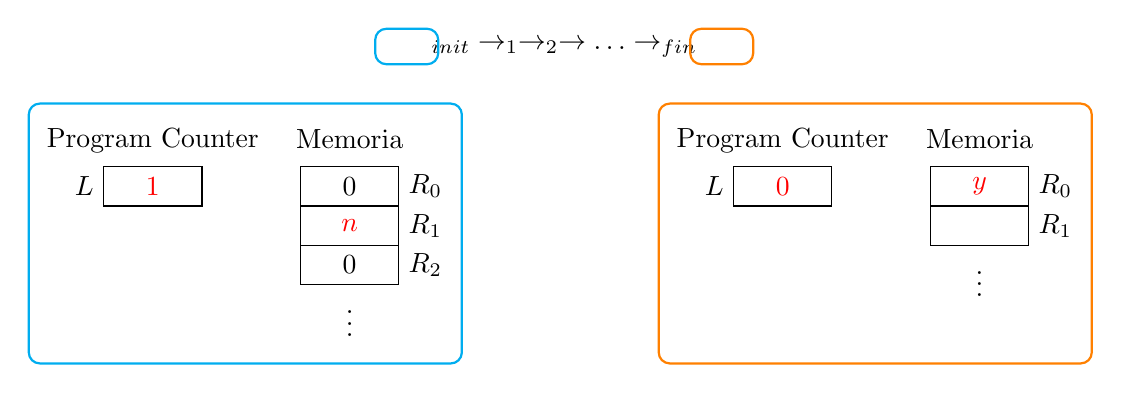
\begin{tikzpicture}

    \node at (3.6,2) {$\Stato_{init} \to \Stato_1 \to \Stato_2 \to \dots \to \Stato_{fin}$};

    \draw[cyan,rounded corners,thick]
        (1.2,1.8) rectangle (2,2.25);
    \def\plus{4}
    \draw[orange,rounded corners,thick]
        (1.2+\plus,1.8) rectangle (2+\plus,2.25);

    \def\padding{.1}
    \draw[cyan,rounded corners,thick]
        (-3.1-\padding,-1.9-\padding) rectangle (2.2+\padding,1.2+\padding);

    \node[above] at (.875,.6) {Memoria};

    \draw (.25,0) rectangle (1.5,.5) node[midway] {$0$};
    \node[right] at (1.5,.25) {$R_0$};
    \draw (.25,-.5) rectangle (1.5,0) node[midway] {$\color{red}n$};
    \node[right] at (1.5,-.25) {$R_1$};
    \draw (.25,-1) rectangle (1.5,-.5) node[midway] {$0$};
    \node[right] at (1.5,-.75) {$R_2$};
    
    \node[below] at (.875,-1) {$\vdots$};

    \def\x{2.5}
    \node[above] at (.875-\x,.55) {Program Counter};

    \draw (.25-\x,0) rectangle (1.5-\x,.5) node[midway] {$\color{red}1$};
    \node[left] at (1.5-1.25-\x,.25) {$L$};

    \begin{scope}[xshift=8cm]
        \draw[orange,rounded corners,thick]
        (-3.1-\padding,-1.9-\padding) rectangle (2.2+\padding,1.2+\padding);

        \node[above] at (.875,.6) {Memoria};

        \draw (.25,0) rectangle (1.5,.5) node[midway] {$\color{red}y$};
        \node[right] at (1.5,.25) {$R_0$};
        \draw (.25,-.5) rectangle (1.5,0);
        \node[right] at (1.5,-.25) {$R_1$};
        
        \node[below] at (.875,-.5) {$\vdots$};

        \def\x{2.5}
        \node[above] at (.875-\x,.55) {Program Counter};

        \draw (.25-\x,0) rectangle (1.5-\x,.5) node[midway] {$\color{red}0$};
        \node[left] at (1.5-1.25-\x,.25) {$L$};
    \end{scope}
\end{tikzpicture}
\end{figure}

La semantica di $P$ è:
$$ \semanticaRAM_P:\N\to\N_\perp $$
$$ \semanticaRAM_P(n) = \begin{cases}
\perp & \text{se $P$ va in loop}\\
y & \text{altrimenti}
\end{cases} $$

\subsubsection*{Stato}
Come già anticipato, uno stato è una \quotes{foto} di tutte le componenti della macchina
in un dato istante. Formalmente si definisca uno stato come una funzione:
$$ \Stato:\{L,R_i\}\to\N $$
$$ \Stato(R_j) = \text{contenuto del registro $R_j$ quando la macchina è nello stato 
$\Stato$}$$

I possibili stati della macchina sono:
$$ \text{STATI} = \N^{\{L,R_i\}} $$

Uno stato è finale se $\Stato(L)=0$.

La funzione di inizializzazione $in$, preso l'input del programma, restituisce lo stato
iniziale:
$$ in:\text{DATI}\to\text{STATI} $$
$$ in(n) = \Stato_{init} $$
$$ \Stato_{init}(L) = 1 \qquad\qquad \Stato_{init}(R_i) = \begin{cases}
n & i=1\\
0 & i\neq 1
\end{cases} $$

\subsubsection*{Funzione stato prossimo}
A definire la dinamica del programma è la funzione stato prossimo $\delta$:
$$ \delta : \text{STATI}\times\text{PROG}\to\text{STATI}_\perp $$
$$ \delta({\color{red}\Stato},P) = {\color{blue}\Stato'} $$
$$ {\color{red}\text{Stato attuale}} \qquad {\color{blue}\text{Stato prossimo}} $$

\begin{enumerate}
    \item Se $\Stato(L)=0$ allora $\Stato'=\perp$
    \item Se $\Stato(L)>|P|$ allora $\Stato'(L)=0$ e $\forall i:\Stato'(R_i)=\Stato(R_i)$
    \item Se $1\leq\Stato(L)\leq |P|$: considera la $\Stato(L)$-esima istruzione:
        \begin{enumerate}
            \item Se $R_k \leftarrow R_k +/\dotminus 1$ allora:
                \begin{itemize}
                    \item $\Stato'(R_k) = \Stato(R_k)+/\dotminus 1$
                    \item $\Stato'(L) = \Stato(L)+1$
                    \item $\forall i:i\neq k \quad \Stato'(R_i) = \Stato(R_i)$
                \end{itemize}
            \item Se $\goto{R_k}{m}$ allora:
                \begin{itemize}
                    \item Se $\Stato(R_k)=0$ allora $\Stato'(L) = m$
                    \item Altrimenti $\Stato'(L) = \Stato(L)+1$
                \end{itemize}
        \end{enumerate}
\end{enumerate}

\subsubsection*{Esempio di programma}
\vspace{-1em}
\begin{minipage}{.48\textwidth}
    \begin{align}
        P \equiv\ & \goto{R_1}{6}       \notag\\
        & R_0 \leftarrow R_0+1          \notag\\
        & R_0 \leftarrow R_0+1          \notag\\[-.3em]
        & R_1 \leftarrow R_1\dotminus 1 \notag\\
        & \goto{R_2}{1}                 \notag\\[-.3em]
        & R_1 \leftarrow R_1\dotminus 1 \notag
    \end{align}
\end{minipage}
\begin{minipage}{.48\textwidth}
    $ \semanticaRAM_P(n) = 2n $
\end{minipage}

\subsubsection*{Aritmetizzazione di un programma RAM}
Essendo un programma RAM una lista di istruzioni, per poter codificare e decodificare
dei programmi basterà trovare una funzione $Ar$ che codifica le singole istruzioni, 
ottenenendo una lista di numeri che si può facilmente codificare con $\cantor{\ ,\ }$:
\begin{figure}[H]
    \centering
    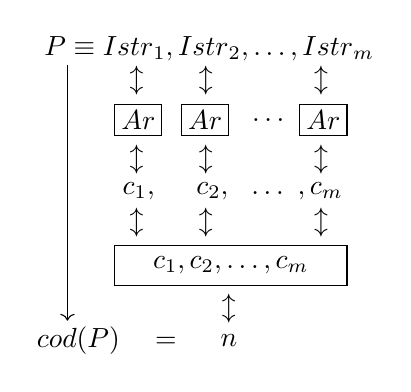
\begin{tikzpicture}
    \node at (0,0)
        {$ P \equiv \text{Istr}_1,\text{Istr}_2,\dots,\text{Istr}_m$};
    \node at (.25,-.4) 
        {$\updownarrow \qquad \updownarrow \qquad \ \ \ \ \ \updownarrow$};
    
    \draw (-1.2,-1.1) rectangle (-.6,-.7) node[midway] {$Ar$};
    \begin{scope}[xshift=.85cm]
        \draw (-1.2,-1.1) rectangle (-.6,-.7) node[midway] {$Ar$};
    \end{scope}
    \begin{scope}[xshift=2.35cm]
        \draw (-1.2,-1.1) rectangle (-.6,-.7) node[midway] {$Ar$};
    \end{scope}
    \node at (.75,-.9) {$\dots$};

    \node at (.25,-1.4) 
        {$\updownarrow \qquad \updownarrow \qquad \ \ \ \ \ \updownarrow$};
    \node at (.3,-1.8) 
        {$c_1,\ \ \ \ c_2, \ \ \dots \  ,c_m$};
    \node at (.25,-2.2) 
        {$\updownarrow \qquad \updownarrow \qquad \ \ \ \ \ \updownarrow$};
    \draw (-1.2,-3) rectangle (1.75,-2.5) node[midway] 
        {$\cantor{c_1,c_2,\dots,c_m}$};
    \node at (.25,-3.3) {$\updownarrow$};
    \node at (.25,-3.7) {$n$};
    \node at (-1.3,-3.7) {$cod(P) \quad =$};
    \draw [->] (-1.8,-.2) -- (-1.8,-3.45);

\end{tikzpicture}
\end{figure}

L'associazione biunivoca di un numero ad una struttura si dice aritmetizzazione o
Gödellizzazione.

\subsubsection*{Aritmetizzazione delle istruzioni RAM}
Per poter aritmetizzare un'istruzione RAM c'è bisogno di una funzione che:
$$ Ar:\text{Istr}\to\N \quad , \quad Ar^{-1}:\N\to\text{Istr} $$
Il linguaggio RAM è formato da tre tipi di istruzioni; si può quindi ottenere la
seguente aritmetizzazione:
$$ \begin{aligned}
    Ar(R_k\leftarrow R_k+1) &= 3k\\
    Ar(R_k\leftarrow R_k\dotminus1) &= 3k+1\\
    Ar(\goto{R_k}{m}) &= 3\cantor{k,m}-1
\end{aligned} $$
Mentre per calcolare la sua inversa $Ar^{-1}$, ovvero a partire da un numero $n$ decodificare
l'istruzione:
\begin{itemize}
    \item Se $n\bmod{3}=0$:
        \begin{itemize}
            \begin{minipage}{.35\textwidth}
                \item È un'istruzione di primo tipo
                \item $n=3k$
            \end{minipage}
            \begin{minipage}{.3\textwidth}
                $\Rightarrow \qquad R_{\frac{n}{3}} \leftarrow R_{\frac{n}{3}}+1$
            \end{minipage}
        \end{itemize}
    \item Se $n\bmod{3}=1$:
        \begin{itemize}
            \begin{minipage}{.35\textwidth}
                \item È un'istruzione di secondo tipo
                \item $n=3k+1$
            \end{minipage}
            \begin{minipage}{.3\textwidth}
                $\Rightarrow \qquad R_{\frac{n-1}{3}} \leftarrow R_{\frac{n-1}{3}}\dotminus1$
            \end{minipage}
        \end{itemize}
    \item Se $n\bmod{3}=2$:
        \begin{itemize}
            \begin{minipage}{.35\textwidth}
                \item È un'istruzione di terzo tipo
                \item $n=3\cantor{k,m}-1$
            \end{minipage}
            \begin{minipage}{.5\textwidth}
                $\Rightarrow \qquad \goto{R_{\sx(\frac{n+1}{3})}}{\dx(\frac{n+1}{3})}$
            \end{minipage}
        \end{itemize}
\end{itemize}

\subsubsection*{Potenza computazionale del sistema RAM}
$$ \begin{aligned}
        F(\RAM) &= \{f\in\N_\perp^\N:\exists P \in \PROG: \semanticaRAM_P=f\}\\
                &= \{\semanticaRAM_P:P\in\PROG\} \subset \N_\perp^\N \\
                \multispan2{Vista la possibilità di rappresentare un programma
                 con un numero si ha:\hfill}\notag\\
                 &= \{\semanticaRAM_i:i\in\N\}
\end{aligned} $$
Dove $\semanticaRAM_i$ è la semantica del programma la cui codifica è $i$.
\subsubsection*{Conclusioni}
Nelle ultime sezioni si è mostrata una biezione tra programmi RAM (PROG) e numeri
($\N$):
    \begin{itemize}
        \item Da programmi a numeri:
            $cod(P)=\cantor{Ar(\text{Istr}_1),Ar(\text{Istr}_2),\dots,Ar(\text{Istr}_m)}$
        \item Da numeri a programmi: si decodifichi la lista di numeri e si applichi su
            ogni numero $Ar^{-1}$
    \end{itemize}
Per quanto riguarda i programmi RAM, \textbf{si può quindi affermare che}:
$$ F(\RAM) \sim \N \nsim \N^\N_\perp $$
e quindi esistono problemi non risolubili automaticamente da una macchina RAM.
\subsubsection{Sistema di calcolo WHILE}
Per mostrare se il concetto di calcolabilità è legato al sistema di calcolo o meno,
se ne vedrà uno più sofisticato: quello WHILE.
\subsubsection*{Macchina WHILE}
La macchina WHILE è più semplice di quella RAM; è formata infatti da un'unica memoria
con un numero finito di registri:
$$\text{Memoria: } x_0,x_1,x_2,\dots,x_{20}$$
\begin{itemize}
    \item $x_i$ è un generico registro di memoria detto variabile:
        \begin{itemize}
            \item $x_0$ è la variabile specifica dove verrà deposto l'output del programma
            \item $x_1$ è la variabile specifica dove verrà letto l'input del programma
            \item Ci sono 21 variabili
        \end{itemize}
    \item Non c'è un Program Counter
\end{itemize}

\subsubsection*{Linguaggio WHILE}
La sintassi del linguaggio WHILE è induttiva; le istruzioni, dette comandi, sono:
\begin{itemize}
    \item Comando di assegnamento:
        \begin{enumerate}
            \item $x_k := 0$
            \item $x_k := x_j+1$
            \item $x_k := x_j\dotminus 1$
        \end{enumerate}
    \item Comando WHILE:
        \begin{enumerate}
            \item $\while{x_k} C$
        \end{enumerate}
    \item Comando composto:
        \begin{enumerate}
            \item $\textbegin C_ 1; \ C_2; \ \dots; \ C_m; \textend$
        \end{enumerate}
    \end{itemize}
dove $C_i$ è un comando WHILE.

Un programma WHILE è un comando composto.

\subsubsection*{Semantica programma WHILE}
La semantica di un programma $W$ è la funzione
    $$\semanticaWHILE_W:\N\to\N_\perp$$
\subsubsection*{Esempio di programma}
\vspace{-1em}
\begin{minipage}{.34\textwidth}
    \begin{align}
        W \equiv\ & \textbegin                      \notag\\[-.3em]
        & \qquad x_2 := x_1+1;                      \notag\\[-.3em]
        & \qquad x_2 := x_2\dotminus 1;             \notag\\[-.3em]
        & \qquad \while{x_1}                        \notag\\[-.3em]
        & \qquad\qquad \textbegin                   \notag\\[-.3em]
        & \qquad\qquad\qquad x_0 := x_0+1;          \notag\\[-.3em]
        & \qquad\qquad\qquad x_1 := x_1\dotminus 1; \notag\\[-.3em]
        & \qquad\ \ \ \ \ \textend                  \notag\\[-.3em]
        & \qquad \while{x_2}                        \notag\\[-.3em]
        & \qquad\qquad \textbegin                   \notag\\[-.3em]
        & \qquad\qquad\qquad x_0 := x_0+1;          \notag\\[-.3em]
        & \qquad\qquad\qquad x_2 := x_2\dotminus 1; \notag\\[-.3em]
        & \qquad\ \ \ \ \ \textend                  \notag\\[-.3em]
        & \hspace{-.5em}\textend                            \notag
    \end{align}
\end{minipage} \hspace{1em}
\begin{minipage}{.6\textwidth}
    $\qquad\qquad\ \ \ \semanticaWHILE_W(n) = 2n $
\end{minipage}

\subsubsection*{W-PROG e induzione}
Sia W-PROG l'insieme dei programmi WHILE. La sua definizione è induttiva; per dimostrare
una proprietà $P$ su W-PROG sarà quindi naturale farlo tramite induzione.

\subsubsection*{Stato}
Siccome la macchina WHILE è composta solo da 21 variabili, uno stato della macchina è
una lista di 21 numeri:
$$ \text{STATO} = (c_0,c_1,\dots,c_{20}) $$
$$ c_i = \text{contenuto di $x_i$} $$
$$ \text{W-STATI} = \N^{21} $$
$$ \underbar{$x$}\in\N^{21} $$

La funzione $W$-$in:\N\to\N^{21}$ restituisce lo stato iniziale del programma $W$:
$$ W\text{-}in(n) = (0,n,0,\dots,0) $$

\subsubsection*{Funzione stato prossimo}
Si definisca la funzione stato prossimo e quindi la semantica operazionale:
$$\opsemWHILE{\ }{\ }: \text{W-COM}\times\text{W-STATI}\to\text{W-STATI}_\perp$$
dato un comando $C$ e uno stato $\underbar{x}$:
$$ \opsemWHILE{C}{\sottolinea{x}} = \sottolinea{y} $$
dove $\sottolinea{y}$ è lo stato prossimo di $\sottolinea{x}$ a seguito dell'esecuzione del
comando $C$.

Si veda ora la definizione induttiva della semantica operazionale:
\begin{itemize}
    \item BASE: Assegnamenti
        \begin{itemize}
            \item $\opsemWHILE{x_k:=0}{\sottolinea{x}} = \sottolinea{y}$ con
                $y_i = \begin{cases}
                    x_i & i\neq k\\
                    0 & i= k\\
                \end{cases}$
            \item $\opsemWHILE{x_k:=x_j \pm 1}{\sottolinea{x}} = \sottolinea{y}$ con
                $y_i = \begin{cases}
                    x_i & i\neq k\\
                    x_j\pm 1 & i= k\\
                \end{cases} \hfill \text{(con $\pm$ si intende $+$ o $\dotminus$)}$
        \end{itemize}
    \item PASSO: Comando composto
        \begin{itemize}
            \item $
                \opsemWHILE{\textbegin C_1 \ ; \ \dots \ ; \ C_m\textend}{\sottolinea{x}}
                = \opsemWHILE{C_m}{
                    \dots(
                        \opsemWHILE{C_2}{
                            \opsemWHILE{C_1}{\sottolinea{x}}
                        }
                    )\dots
                }$
            \item[]\hspace{14.1em}$=\opsemWHILEnoP{C_m}\circ\hdots\circ\opsemWHILEnoP{C_1}(\sottolinea{x})$
            \item[]\hspace{14.1em}$=\sottolinea{y}$
        \end{itemize}
    \item PASSO: Comando WHILE
        \begin{itemize}
            \item $
            \opsemWHILE{\while{x_n} C}{\sottolinea{x}} =
            \opsemWHILE{C}{
                \dots(
                \opsemWHILE{C}{
                    \opsemWHILE{C}{\sottolinea{x}}
                })
                \dots
            }=\sottolinea{y}
            $
            \item[]\hspace{11.7em}$=
                \begin{cases}
                    \opsemWHILEnoP{C}^e(\sottolinea{x}) & e=
                    \mu t(\text{componente $k$ di $\opsemWHILEnoP{C}^t(\sottolinea{x})=0$})\\
                    \perp & \text{altrimenti (se non esiste $e)$}
                \end{cases}
            $
            \\[.6em]dove $\mu t (\text{condizione}) = \underset{t}{\min}\{\text{condizione vera\}}$
        \end{itemize}
\end{itemize}
Si può quindi definire la semantica di un programma $W$:
$$\semanticaWHILE_W(n) = \text{Pro}(0,\opsemWHILE{W}{\text{$W$-$in$}(n)})$$
dove Pro è la funzione proiezione:
$$ \text{Pro}(i,(x_0,x_1,\dots,x_m)) = x_i $$

\subsubsection*{Potenza computazionale del sistema WHILE}
$$ \begin{aligned}
    F(\text{WHILE}) &= \{ f\in\N^\N_\perp : \exists W\in \text{W-PROG}:f=\semanticaWHILE_W \}\\
    &= \{ \semanticaWHILE_W : W \in \text{W-PROG} \} 
    \end{aligned}
$$

\subsubsection{Traduzione}
Dati i sistemi di calcolo $\SC_1$ e $\SC_2$, una traduzione da $\SC_1$ a $\SC_2$ è una funzione
$$ T:\SC_1\text{-PROG}\to\SC_2\text{-PROG} $$
tale che $T$ sia:
\begin{enumerate}
    \item Programmabile: è programmabile effettivamente
    \item Completa: traduce ogni programma
    \item Corretta: mantiene la semantica:
        $\forall P\in\SC_1\text{-PROG} \quad \semanticaRAM_{T(P)}=\semanticaWHILE_{P}$
\end{enumerate}
\subsubsection{Confronto tra F(RAM) e F(WHILE)}
Si prendano due sistemi di calcolo $\SC_1$ e $\SC_2$ con le rispettive potenze computazionali:
$$ F(\SC_1) = \{\semanticaRAM_{P_1}:P_1\in\SC_1\text{-PROG}\} $$
$$ F(\SC_2) = \{\semanticaWHILE_{P_2}:P_2\in\SC_2\text{-PROG}\} $$

Si vuole mostrare che $F(\SC_1)\subseteq F(\SC_2)$, ovvero che $\SC_1$ non è più potente di $\SC_2$;
per farlo bisogna dimostrare che:
\begin{table}[H]
    \centering
    \begin{tabular}{c}
        $\forall f \in F(\SC_1) \quad f\in F(\SC_2)$\\[1em]
        \rotatebox[origin=c]{90}{$\equiv$}\\[1em]
        $\exists P_1\in\SC_1\text{-PROG}:f=\semanticaRAM_{P_1}
    \ \Rightarrow \ \exists P_2\in\SC_2\text{-PROG}:f=\semanticaWHILE_{P_2}$
    \end{tabular}
\end{table}
In altre parole, per ogni programma di $\SC_1$ ne esiste uno equivalente in $\SC_2$.
\\
\begin{theorem}
    Se esiste una traduzione $T$ da $\SC_1$ a $\SC_2$, allora $F(\SC_1)\subseteq F(\SC_2)$.
\end{theorem}
\begin{proof}
    Si prenda una funzione $f$ tale che:
    $$ f\in F(\SC_1) $$
    Si ha quindi che esiste un programma in $\SC_1\text{-PROG}$ che può calcolare $f$:
    \begin{equation} \label{eq:traduzione_proof1}
        \exists P\in\SC_1\text{-PROG}:f=\semanticaWHILE_P
    \end{equation}
    Si prenda la traduzione $T$ da $\SC_1$ a $\SC_2$; vista la completezza di $T$ si ha che:
    \begin{equation} \label{eq:traduzione_proof2}
        T(P)\in\SC_2\text{-PROG}
    \end{equation}
    e vista la correttezza si ha che:
    \begin{equation} \label{eq:traduzione_proof3}
        \semanticaRAM_{T(P)}=\semanticaWHILE_P\underset{(\ref{eq:traduzione_proof1})}{=}f
    \end{equation}
    Si ha quindi che esiste un programma $T(P)$ in $\SC_2$-PROG (\ref{eq:traduzione_proof2})
    la cui semantica è $f$ (\ref{eq:traduzione_proof3}). Si può concludere che:
    $$ f\in F(\SC_2) $$ 
\end{proof}